\subsection{Quản lý hồ sơ cá nhân}
\label{subsec:req_profile}
\label{subsec:module_profile}

\subsubsection{Mục tiêu và yêu cầu chức năng}

HRM quản lý dữ liệu hồ sơ chính thức; MyHCMUT Mobile cung cấp giao diện native để tra cứu, chỉnh sửa, phản hồi và xem lịch sử. Chính sách do HRM cung cấp xác định cách xử lý từng trường: cập nhật trực tiếp hoặc gửi đề xuất cần thẩm định. Hai loại trường có thể cùng xuất hiện trong một lần thao tác. Mobile dùng chính sách để dựng biểu mẫu; HRM kiểm tra lại quyền, dữ liệu và chính sách khi ghi nhận.

Thông tin được phân thành ba nhóm giao diện trong Bảng~\ref{tab:profile_groups}. Chuyên viên TCNS có quyền thẩm định đối chiếu nội dung đề xuất với dữ liệu hiện tại và minh chứng, sau đó xử lý từng nội dung được phân công.

\begin{table}[H]
\centering
\small
\caption{Phân nhóm danh mục thông tin hồ sơ nhân sự}
\label{tab:profile_groups}
\vspace{0.15cm}
\begin{tabularx}{\textwidth}{|L{4.2cm}|Y|}
\hline
\textbf{Nhóm giao diện} & \textbf{Các danh mục thông tin thành phần} \\
\hline
\textbf{Cá nhân và gia đình} & Thông tin cá nhân cơ bản; Địa chỉ cư trú (thường trú, tạm trú); Quan hệ gia đình (thân nhân, người phụ thuộc). \\
\hline
\textbf{Công tác và đào tạo} & Quá trình công tác / vị trí việc làm hiện tại; Trình độ học vấn, văn bằng chứng chỉ và quá trình đào tạo, bồi dưỡng chuyên môn. \\
\hline
\textbf{Chế độ và thông tin khác} & Quá trình lương và phụ cấp; Khen thưởng; Kỷ luật; Thông tin sức khỏe; Kê khai tài sản / thu nhập. \\
\hline
\end{tabularx}
\end{table}

\begin{table}[H]
\centering
\small
\caption{Yêu cầu chức năng nhóm quản lý hồ sơ cá nhân}
\label{tab:fr_profile}
\begin{tabularx}{\textwidth}{|L{1.8cm}|L{3.5cm}|L{2.5cm}|Y|}
\hline
\textbf{Mã FR} & \textbf{Chức năng} & \textbf{Tác nhân} & \textbf{Mô tả và ràng buộc nghiệp vụ} \\
\hline
FR-PRO-01 & Tra cứu hồ sơ & Nhân sự & Xem các danh mục thông tin lý lịch cá nhân do HRM cung cấp. \\
\hline
FR-PRO-02 & Cập nhật hồ sơ & Nhân sự & Chỉnh sửa bằng biểu mẫu native theo chính sách từng trường; HRM kiểm tra quyền và dữ liệu để cập nhật trực tiếp hoặc tiếp nhận đề xuất kèm minh chứng. \\
\hline
FR-PRO-03 & Thẩm định đề xuất & Chuyên viên TCNS & Đối với đề xuất cần thẩm định, xem xét thông tin sai khác, đối chiếu minh chứng và phê duyệt hoặc từ chối theo thẩm quyền. \\
\hline
FR-PRO-04 & Gửi phản hồi hồ sơ & Nhân sự & Gửi nội dung phản hồi kèm ít nhất một tài liệu minh chứng về danh mục hồ sơ; phản hồi không tự cập nhật dữ liệu chính thức. \\
\hline
FR-PRO-05 & Xem lịch sử hồ sơ & Nhân sự & Quan sát yêu cầu và nhật ký cập nhật; đối chiếu dữ liệu ban đầu với dữ liệu mới hoặc đề xuất theo từng trường, kèm trạng thái xử lý do HRM trả về. \\
\hline

\end{tabularx}
\end{table}

\subsubsection{Đặc tả Use Case}

UC-PRO-01 đến UC-PRO-05 lần lượt tương ứng FR-PRO-01 đến FR-PRO-05. Hình~\ref{fig:uc_profile} minh họa các nhánh nghiệp vụ; UC-PRO-05 bổ sung chức năng lịch sử.

\begin{figure}[H]
\centering
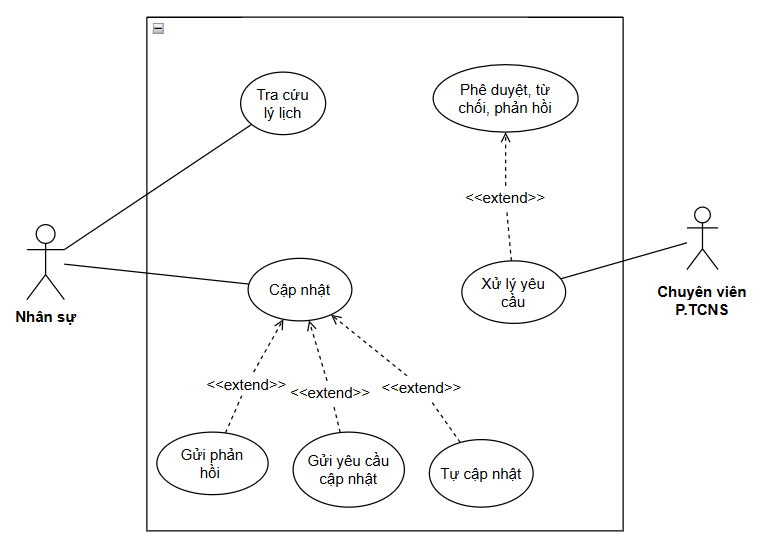
\includegraphics[width=\linewidth]{image/usecase/UC_PROFILE.png}
\caption{Sơ đồ Đặc tả Use case nhóm Quản lý hồ sơ cá nhân}
\label{fig:uc_profile}
\end{figure}

\usecasespec{
  id={UC-PRO-01},
  name={Tra cứu hồ sơ nhân sự},
  shortname={Tra cứu hồ sơ},
  actor={Nhân sự},
  desc={Cho phép nhân sự tra cứu các danh mục thông tin lý lịch cá nhân được cung cấp bởi hệ thống HRM.},
  pre={Nhân sự đã đăng nhập thành công vào ứng dụng MyHCMUT Mobile.},
  trigger={Người dùng chọn mục ``Hồ sơ cá nhân'' trên ứng dụng di động.},
  mainflow={
    1. Người dùng mở giao diện hồ sơ cá nhân trên ứng dụng. \newline
    2. Ứng dụng hiển thị thông tin tổng quan và ba nhóm giao diện chính. \newline
    3. Người dùng lựa chọn nhóm và danh mục thông tin cần xem. \newline
    4. Ứng dụng tải và hiển thị chi tiết các trường dữ liệu tương ứng từ hệ thống HRM.
  },
  altflow={
    - \textit{Luồng 2a (Làm mới dữ liệu):} Người dùng thực hiện làm mới để yêu cầu ứng dụng tải dữ liệu mới nhất từ hệ thống HRM.
  },
  exflow={
    - \textit{Ngoại lệ 4a (Lỗi kết nối):} Khi không thể tải dữ liệu từ hệ thống HRM, ứng dụng sử dụng dữ liệu hồ sơ đã lưu tạm trước đó nếu có và thông báo trạng thái kết nối cho người dùng. Nếu chưa có dữ liệu lưu tạm, ứng dụng thông báo không thể tải dữ liệu.
  },
  post={Người dùng xem được dữ liệu hồ sơ mới nhất tải được từ HRM hoặc dữ liệu đã lưu tạm gần nhất khi không thể kết nối.},
  label={tab:uc_pro_01}
}

\usecasespec{
  id={UC-PRO-02},
  name={Cập nhật hồ sơ cá nhân},
  shortname={Cập nhật hồ sơ},
  actor={Nhân sự},
  desc={Cho phép nhân sự cập nhật thông tin hồ sơ theo phạm vi quyền; HRM ghi nhận trực tiếp các thông tin được phép và tiếp nhận đề xuất đối với thông tin cần thẩm định.},
  pre={Nhân sự đã đăng nhập vào MyHCMUT Mobile và đang xem hồ sơ của bản thân.},
  trigger={Người dùng chọn chức năng cập nhật tại danh mục thông tin tương ứng.},
  mainflow={
    1. Người dùng chọn cập nhật thông tin hồ sơ. \newline
    2. Ứng dụng tải dữ liệu hiện tại và chính sách cập nhật từ HRM, sau đó mở biểu mẫu Flutter của danh mục được hỗ trợ. \newline
    3. Người dùng điều chỉnh các thông tin cần thay đổi và cung cấp tài liệu minh chứng đối với những nội dung yêu cầu minh chứng. \newline
    4. Ứng dụng kiểm tra dữ liệu đầu vào và minh chứng theo chính sách, chỉ gửi những trường thực sự thay đổi khi người dùng xác nhận. \newline
    5. HRM kiểm tra quyền, tính hợp lệ của dữ liệu và chính sách áp dụng cho từng trường thông tin. \newline
    6. Các trường được phép tự cập nhật được ghi nhận trực tiếp; các trường cần thẩm định được ghi nhận thành nội dung đề xuất chờ xử lý. \newline
    7. Hệ thống phản hồi kết quả để người dùng theo dõi thông tin hoặc trạng thái đề xuất tương ứng.
  },
  exflow={
    - \textit{Ngoại lệ 4a (Thiếu tài liệu minh chứng):} Khi thiếu tài liệu minh chứng đối với nội dung yêu cầu minh chứng, hệ thống thông báo để người dùng bổ sung trước khi tiếp nhận nội dung tương ứng. \newline
    - \textit{Ngoại lệ 4b (Mất kết nối):} Ứng dụng thông báo lỗi; không coi dữ liệu đang nhập là thay đổi đã được HRM lưu. Khi chưa xác định kết quả gửi, người dùng cần kiểm tra hồ sơ hoặc lịch sử trước khi gửi lại. \newline
    - \textit{Ngoại lệ 5a (Không đáp ứng điều kiện nghiệp vụ):} Khi tồn tại điều kiện nghiệp vụ không cho phép tiếp nhận thay đổi, hệ thống từ chối thao tác và phản hồi nguyên nhân cho người dùng.
  },
  post={Thông tin được phép đã được cập nhật vào hồ sơ; các thông tin cần thẩm định được ghi nhận thành đề xuất chờ xử lý.},
  label={tab:uc_pro_02}
}

\usecasespec{
  id={UC-PRO-03},
  name={Thẩm định thay đổi hồ sơ},
  shortname={Thẩm định thay đổi hồ sơ},
  actor={Chuyên viên Phòng Tổ chức Nhân sự có thẩm quyền},
  desc={Cho phép chuyên viên TCNS có thẩm quyền đối chiếu nội dung đề xuất với dữ liệu hiện tại và tài liệu minh chứng, sau đó xử lý các nội dung thay đổi theo phạm vi được phân công.},
  pre={Chuyên viên đã đăng nhập và tài khoản được phân quyền thẩm định hồ sơ nhân sự.},
  trigger={Chuyên viên mở danh sách các đề xuất cập nhật hồ sơ đang chờ xử lý.},
  mainflow={
    1. Chuyên viên mở danh sách đề xuất cập nhật hồ sơ chờ xử lý. \newline
    2. Chọn một đề xuất cụ thể để xem chi tiết. \newline
    3. Ứng dụng hiển thị thông tin hiện tại và nội dung đề xuất để chuyên viên đối chiếu, kèm tài liệu minh chứng tương ứng. \newline
    4. Chuyên viên lựa chọn phê duyệt hoặc từ chối đối với từng nội dung thay đổi theo phạm vi được cấp quyền. \newline
    5. Đối với thao tác từ chối, ứng dụng yêu cầu chuyên viên nhập lý do. \newline
    6. Hệ thống ghi nhận kết quả xử lý của từng nội dung. Khi toàn bộ nội dung thuộc đề xuất đã được xử lý, trạng thái của đề xuất được cập nhật tương ứng và các thay đổi được chấp thuận được phản ánh vào hồ sơ. \newline
    7. Kết quả xử lý được ghi nhận để người đề xuất theo dõi.
  },
  altflow={
    - \textit{Luồng 4a (Xử lý từng phần):} Một đề xuất có thể được xử lý từng phần; các nội dung đã được xử lý được ghi nhận kết quả trong khi các nội dung còn lại tiếp tục chờ xử lý.
  },
  exflow={
    - \textit{Ngoại lệ 4a (Trạng thái hoặc quyền xử lý thay đổi):} Khi thao tác không còn hợp lệ do trạng thái đề xuất đã thay đổi hoặc người dùng không còn quyền xử lý nội dung tương ứng, hệ thống từ chối thao tác và yêu cầu làm mới trạng thái hiện tại.
  },
  post={Kết quả xử lý của từng nội dung được ghi nhận; khi toàn bộ nội dung đã được xử lý, đề xuất đạt trạng thái kết thúc tương ứng và dữ liệu hồ sơ phản ánh các thay đổi đã được chấp thuận.},
  label={tab:uc_pro_03}
}

\usecasespec{
 id={UC-PRO-04}, name={Gửi phản hồi hồ sơ}, shortname={Gửi phản hồi}, actor={Nhân sự},
 desc={Ghi nhận phản hồi liên quan đến một danh mục hồ sơ bằng giao diện native.},
 pre={Người dùng đã đăng nhập và có quyền gửi phản hồi tại danh mục tương ứng.},
 trigger={Người dùng chọn gửi phản hồi trong menu thao tác hồ sơ.},
 mainflow={1. Ứng dụng mở biểu mẫu phản hồi của danh mục được chọn. \newline
 2. Người dùng nhập nội dung phản hồi và đính kèm ít nhất một tài liệu minh chứng. \newline
 3. Ứng dụng gửi nội dung theo hợp đồng API phản hồi của HRM. \newline
 4. HRM kiểm tra quyền và dữ liệu, ghi nhận phản hồi rồi trả kết quả. \newline
 5. Ứng dụng thông báo kết quả; người dùng theo dõi tại lịch sử hồ sơ.},
 exflow={- Thiếu nội dung hoặc minh chứng: yêu cầu bổ sung trước khi gửi. \newline
 - Dữ liệu không hợp lệ, quyền thay đổi hoặc lỗi kết nối: hiển thị lỗi; không thông báo gửi thành công khi backend chưa xác nhận.},
 post={Phản hồi hợp lệ được ghi nhận; dữ liệu hồ sơ chính thức không tự thay đổi chỉ vì đã gửi phản hồi.}, label={tab:uc_pro_04}
}
\usecasespec{
 id={UC-PRO-05}, name={Xem lịch sử hồ sơ}, shortname={Xem lịch sử}, actor={Nhân sự},
 desc={Tra cứu các yêu cầu, nội dung thay đổi và nhật ký mà HRM cho phép người dùng xem.},
 pre={Người dùng đã đăng nhập và được truy cập lịch sử hồ sơ tương ứng.},
 trigger={Người dùng chọn mục lịch sử hồ sơ.},
 mainflow={1. Ứng dụng yêu cầu lịch sử từ HRM. \newline
 2. HRM xác định phạm vi dữ liệu theo phiên và quyền, trả yêu cầu cùng nhật ký liên quan. \newline
 3. Ứng dụng trình bày hai nhóm yêu cầu và thay đổi đã ghi nhận, kèm thời điểm, trạng thái và thông tin xử lý được backend trả về. \newline
 4. Người dùng mở chi tiết để quan sát các trường khác nhau, đối chiếu dữ liệu ban đầu với dữ liệu mới hoặc nội dung đề xuất; xem lý do và minh chứng nếu có.},
 altflow={- Không có lịch sử: ứng dụng hiển thị trạng thái danh sách rỗng.},
 exflow={- Không thể tải hoặc không đủ quyền: thông báo lỗi, không diễn giải dữ liệu chưa tải là không có yêu cầu.},
 post={Người dùng xem được lịch sử do HRM cung cấp; thao tác này không thay đổi trạng thái yêu cầu.}, label={tab:uc_pro_05}
}

UC-PRO-05 sử dụng giá trị trước/sau do HRM trả về để đối chiếu từng trường có dữ liệu lịch sử; nội dung chờ duyệt hoặc bị từ chối chưa phải dữ liệu có hiệu lực. Phạm vi chỉnh sửa native gồm thông tin cá nhân, địa chỉ, ngân hàng/bảo hiểm, gia đình, công tác ngoài Trường, đào tạo và kê khai tài sản/thu nhập. Chính sách chỉnh sửa và minh chứng được áp dụng riêng theo danh mục, không mặc định mọi trường đều được sửa hoặc đều cần tệp.

\subsubsection{Biểu đồ hoạt động}

Hình~\ref{fig:act_profile_request} thể hiện cập nhật trực tiếp và thẩm định đề xuất theo từng nhóm trường; cả hai hướng có thể cùng xuất hiện trong một lần cập nhật.

\begin{figure}[H]
\centering
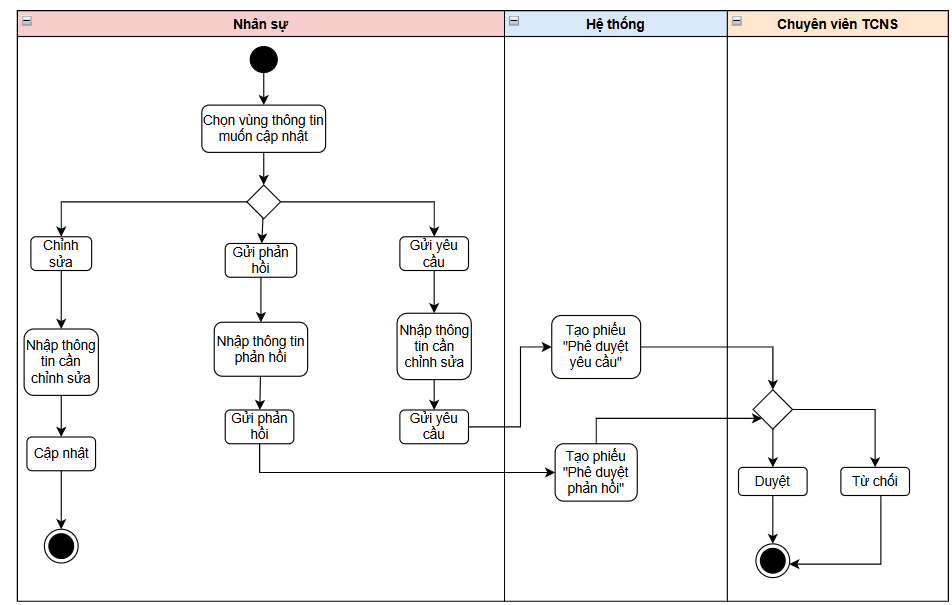
\includegraphics[width=\linewidth]{image/uml/profile_activity.png}
\caption{Biểu đồ hoạt động Quy trình cập nhật hồ sơ cá nhân}
\label{fig:act_profile_request}
\end{figure}

\subsubsection{Biểu đồ tuần tự}

Hình~\ref{fig:seq_profile_request} minh họa lấy dữ liệu/chính sách, gửi nội dung thay đổi và xử lý tại HRM. Hai nhánh cập nhật trực tiếp và đề xuất áp dụng theo trường. Hợp đồng API và truyền tệp được trình bày tại Chương~5.

\begin{figure}[H]
\centering
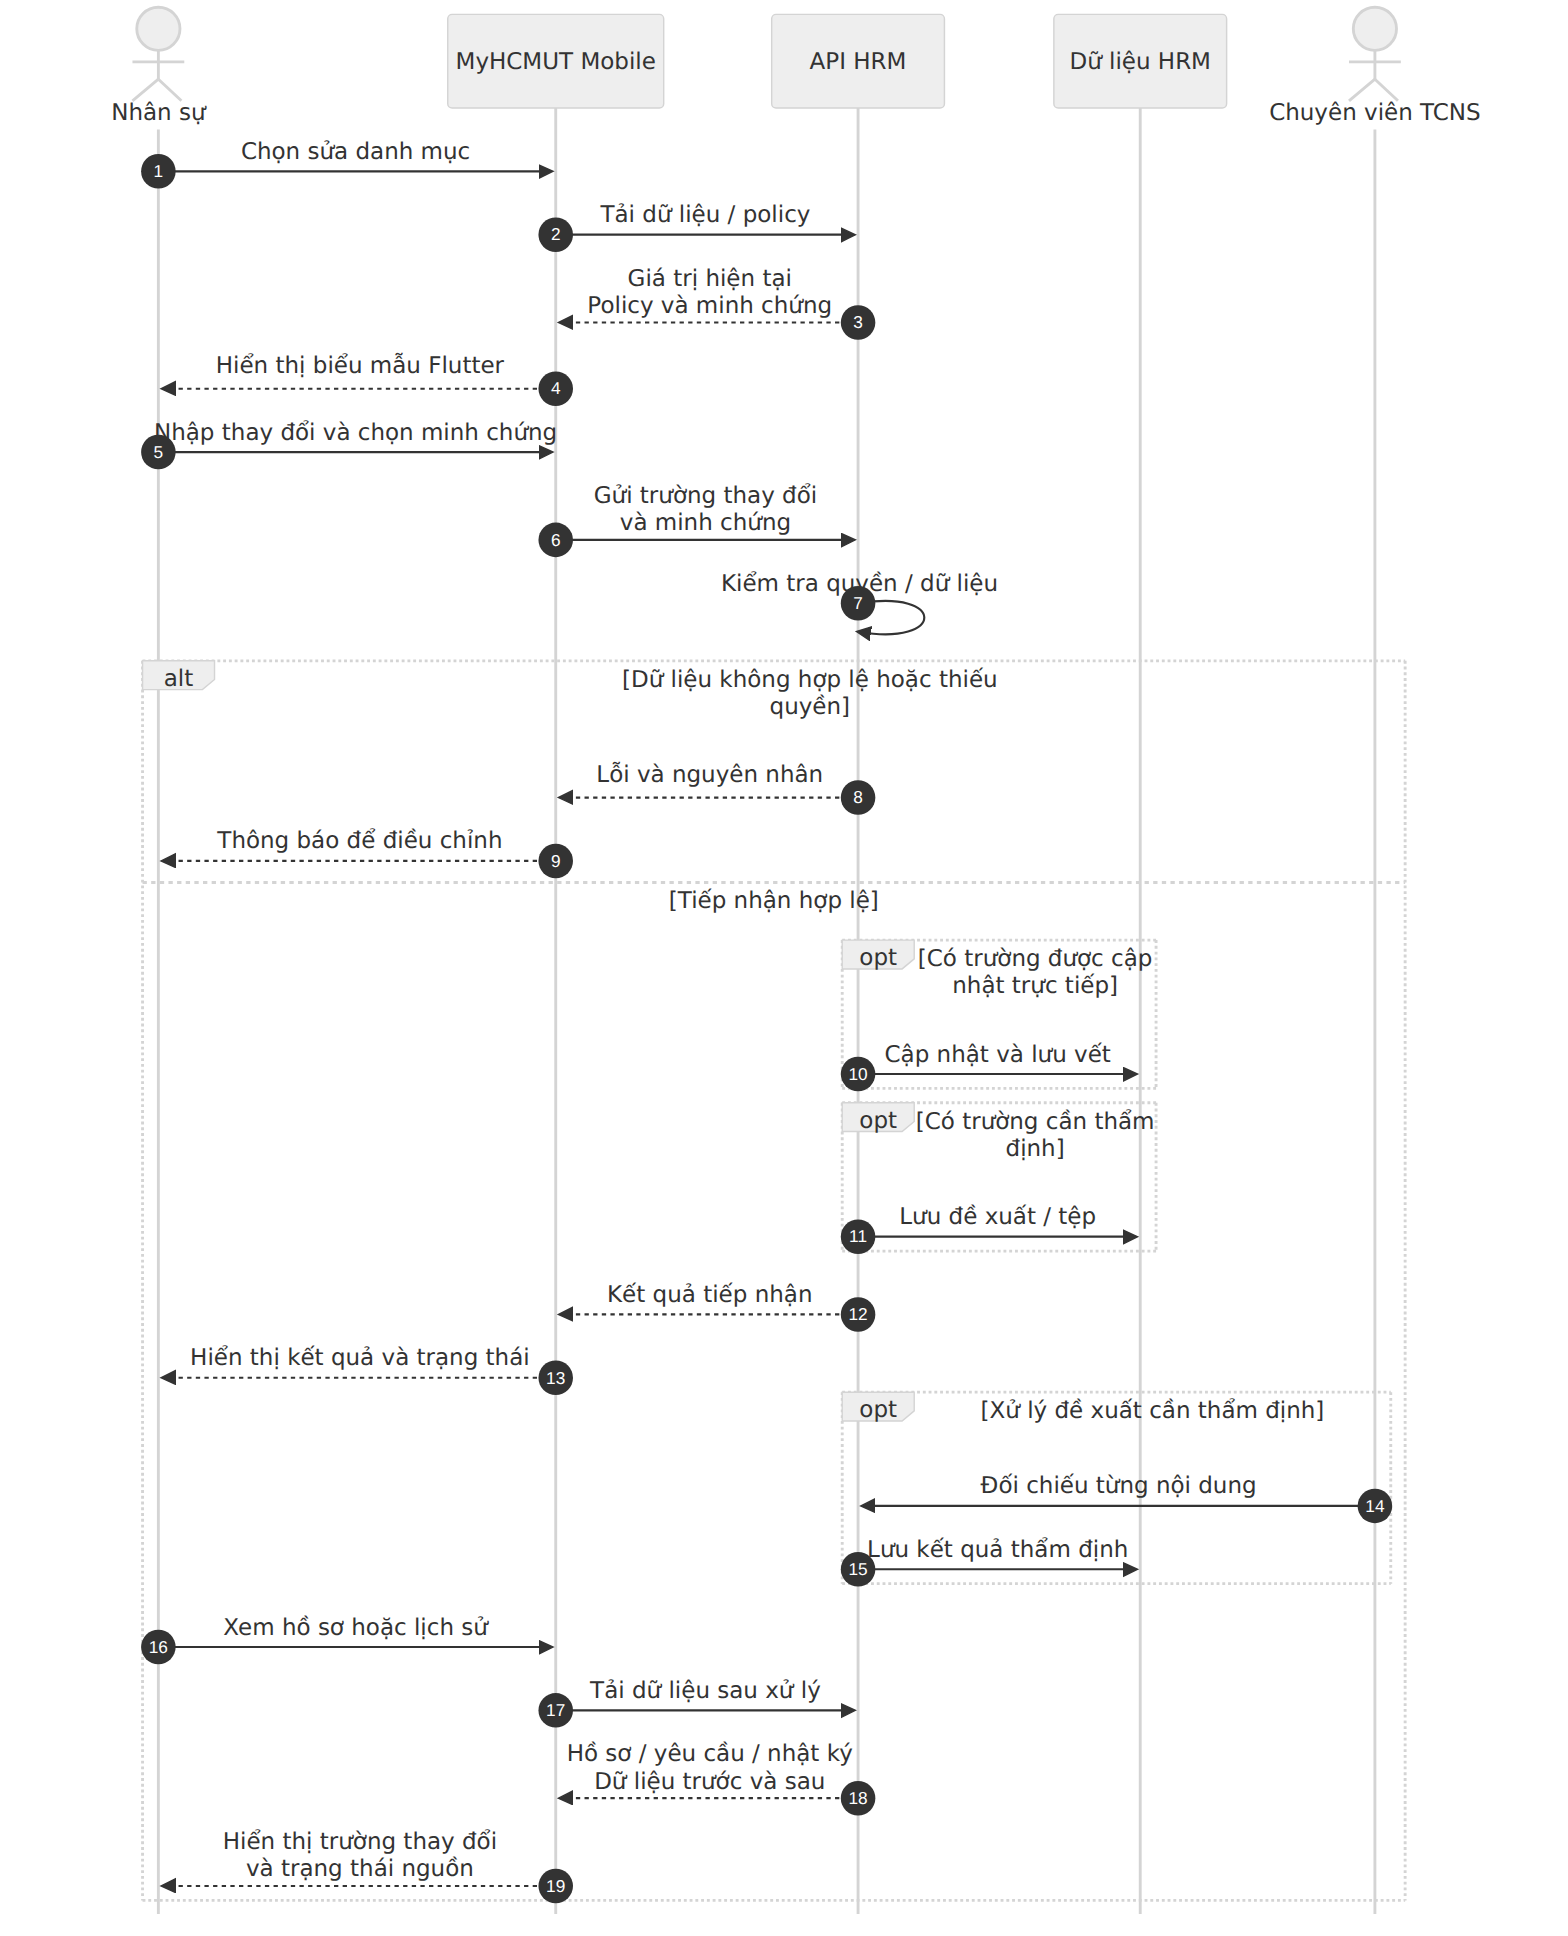
\includegraphics[width=\linewidth]{image/uml/seq_profile_request.png}
\caption{Biểu đồ tuần tự Cập nhật hồ sơ cá nhân}
\label{fig:seq_profile_request}
\end{figure}
